%% ID: inelastic_collision_ZMF
%% TITLE: Inelastic Collision in the ZMF
%% TYPE: question
%% QUESTIONTYPE: numeric
%% CONCEPTS:  energy, momentum, zero_momentum_frame, vectors, resolving_vectors
%% VIDEOS: 
%% LEVEL: 6
%% TOPIC: mechanics/dynamics
%% ORDER: 5

\begin{problem}[Inelastic collision in the ZMF] %A2-2
 {
A collision occurs between two (non-relativistic) bodies of equal mass $m$ and velocity vectors $\vtr{v}_{1}$ and $\vtr{v}_{2}$; how much kinetic energy is available for conversion to other forms of energy? 
A particle of mass $m$ travelling with speed $V$ along the $+x$ direction collides elastically with a stationary particle of mass $2m$.
The particle of mass $m$ is deflected through an angle of $30^{\circ}$.  What are the final velocity vectors of the two particles in the Laboratory frame?
Your answer should be illustrated by appropriate diagrams in both the laboratory and zero momentum frames.}
{\textit{Cambridge University Tripos 1996}}
{

To determine how much kinetic energy is available for other forms of energy, we must find what the minimum kinetic energy the system can have after the collision. To do this, consider the zero momentum frame. If the kinetic energy is minimum in this frame, then it will also be minimum in the laboratory frame, since both masses are equal. The minimum kinetic energy is when the two masses are stuck together. By conservation of momentum and the fact that each particle has the same mass, the final velocity vectors in the ZMF must be opposite to one another. These velocity vectors do not have a minimum value (however they do have a maximum value since the final kinetic energy cannot exceed the initial kinetic energy). Therefore to reduce the overall final kinetic energy we must choose the minimum size for these velocity vectors, i.e. zero. This results in the final system having both particles moving at the same velocity, hence we may now work out the amount of energy that can converted to other forms as follows.

\begin{equation*}total~momentum~before=total~momentum~after\end{equation*}
\begin{equation*}m\vtr{v}_{1}+m\vtr{v}_{2}=2m\vtr{v}_{3}\end{equation*}
\begin{equation*}\vtr{v}_{3}=\frac{1}{2}(\vtr{v}_{1}+\vtr{v}_{2})\end{equation*}

Therefore the final kinetic energy of the system is $\frac{1}{2}\times 2m \times |\vtr{v}_{3}|^2=\frac{1}{4}m|\vtr{v}_{1}+\vtr{v}_{2}|^2$. The initial kinetic energy of the system is simply the sum of the two particles' energies: $\frac{1}{2}m|\vtr{v}_{1}|^2+\frac{1}{2}m|\vtr{v}_{2}|^2$. Therefore the amount of kinetic energy available for conversion to other forms of energy is $\frac{1}{2}m\left(|\vtr{v}_{1}|^2+|\vtr{v}_{2}|^2\right)-\frac{1}{4}m|\vtr{v}_{1}+\vtr{v}_{2}|^2$ which can be rewritten as $\frac{1}{4}m|\vtr{v}_{1}-\vtr{v}_{2}|^2$.

For the next part of the problem, we must consider the laboratory and zero momentum frames. Firstly let us find the speed of the zero momentum frame so that we can draw velocity vectors in it. The total momentum of the system is $mV$ and since the total mass is $3m$ the velocity of the ZMF is $\frac{V}{3}$ along the +ve x-axis. This allows us to draw the velocities before the collision in the ZMF, as in Figure \ref{fig:Tripos_Inelastic_ZMF_1}. Let us call the resultant velocities in the ZMF $v_1$ and $v_2$ for the lighter and heavier masses respectively, at an angle $\phi$ to the horizontal as in Figure \ref{fig:Tripos_Inelastic_ZMF_2}. By conservation of momentum, the total momentum in the ZMF must, as always, sum to zero. This provides us with the equation:

\begin{equation*}mv_1=2mv_2\end{equation*}
\begin{equation}v_1=2v_2\end{equation}


\begin{figure}[h]
	\centering
	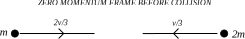
\includegraphics[width=0.6\textwidth]{Tripos_Inelastic_ZMF_1}
	\caption{}
	\label{fig:Tripos_Inelastic_ZMF_1}
\end{figure}

\begin{figure}[h]
	\centering
	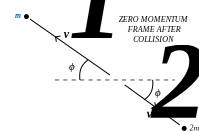
\includegraphics[width=0.6\textwidth]{Tripos_Inelastic_ZMF_2}
	\caption{}
	\label{fig:Tripos_Inelastic_ZMF_2}
\end{figure}


Now we consider conservation of energy in the ZMF:

\begin{equation}\frac{1}{2}m\left(\frac{2V}{3}\right)^2+\frac{1}{2}2m\left(\frac{V}{3}\right)^2=\frac{1}{2}mv_1^2+\frac{1}{2}2mv_2^2\end{equation}

Substituting our value of $v_1$ from equation 1 into equation 2 and simplifying, we find $v_2=\frac{V}{3}$ and hence $v_1=\frac{2V}{3}$. 

It is now easiest to view the laboratory velocities and ZMF velocities on one diagram, using the velocity vector of the ZMF (which is $\frac{V}{3}$) to connect the two, as in Figure \ref{fig:Tripos_Inelastic_ZMF_3}. We also label points at the start and end of vectors to identify particular angles, as in Figure \ref{fig:Tripos_Inelastic_ZMF_3}. 


\begin{figure}[h]
	\centering
	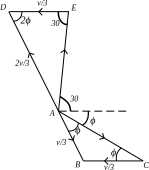
\includegraphics[width=0.4\textwidth]{Tripos_Inelastic_ZMF_3}
	\caption{}
	\label{fig:Tripos_Inelastic_ZMF_3}
\end{figure}

In this diagram we have the final velocity vectors of the light and heavy particles in the laboratory frame as AE and AC respectively. We are told that the angle between AE and the horizontal is $30^\circ$ and we have called the angle between the resultant velocity of the heavy particle and the horizontal $\phi$. From simple geometry we know that angle BAC must also be $\phi$ since ABC is an isosceles triangle. This then allows us to write that angle ADE is $2\phi$. Finally we can deduce that the angle DAE is $150-2\phi$ and so we may use the sine rule on triangle ADE to determine $\phi$ as follows:

\begin{equation*}\frac{\sin{(150-2\phi)}}{v/3}=\frac{\sin{(30)}}{2v/3}\end{equation*}
\begin{equation*}\sin{(2\phi+30)}=\frac{1}{4}\end{equation*}
\begin{equation*}\phi=\frac{1}{2}(\sin^{-1}{(\frac{1}{4})}-30)\end{equation*}

This now allows us to determine the values of the two resultant velocities. The value of AC, the velocity of the particle of mass $2m$, is equal to $\frac{2v}{3}\cos{(\phi)}$ and the value of AE is found by considering the projections of AE and AD onto D:

\begin{equation*}AE\cos{(30)}+\frac{2v}{3}\cos{(2\phi)}=\frac{v}{3}\end{equation*}
\begin{equation*}AE=\frac{2\sqrt{3}}{9}(1-2\cos{(2\phi)})v\end{equation*}

}
\end{problem}